\PassOptionsToPackage{unicode=true}{hyperref} % options for packages loaded elsewhere
\PassOptionsToPackage{hyphens}{url}
%
\documentclass[]{article}
\tracinglostchars=2
\usepackage{lmodern}
\usepackage{amssymb,amsmath}
\usepackage{ifxetex,ifluatex}
\usepackage{fixltx2e} % provides \textsubscript
\ifnum 0\ifxetex 1\fi\ifluatex 1\fi=0 % if pdftex
  \usepackage[T1]{fontenc}
  \usepackage[utf8]{inputenc}
  \usepackage{textcomp} % provides euro and other symbols
\else % if luatex or xelatex
  \usepackage{unicode-math}
  \defaultfontfeatures{Ligatures=TeX,Scale=MatchLowercase}
\fi
% use upquote if available, for straight quotes in verbatim environments
\IfFileExists{upquote.sty}{\usepackage{upquote}}{}
% use microtype if available
\IfFileExists{microtype.sty}{%
\usepackage[]{microtype}
\UseMicrotypeSet[protrusion]{basicmath} % disable protrusion for tt fonts
}{}
\IfFileExists{parskip.sty}{%
\usepackage{parskip}
}{% else
\setlength{\parindent}{0pt}
\setlength{\parskip}{6pt plus 2pt minus 1pt}
}
\usepackage{hyperref}
\hypersetup{
            pdfborder={0 0 0},
            breaklinks=true}
\urlstyle{same}  % don't use monospace font for urls
\usepackage{graphicx,grffile}
\makeatletter
\def\maxwidth{\ifdim\Gin@nat@width>\linewidth\linewidth\else\Gin@nat@width\fi}
\def\maxheight{\ifdim\Gin@nat@height>\textheight\textheight\else\Gin@nat@height\fi}
\makeatother
% Scale images if necessary, so that they will not overflow the page
% margins by default, and it is still possible to overwrite the defaults
% using explicit options in \includegraphics[width, height, ...]{}
\setkeys{Gin}{width=\maxwidth,height=\maxheight,keepaspectratio}
\setlength{\emergencystretch}{3em}  % prevent overfull lines
\providecommand{\tightlist}{%
  \setlength{\itemsep}{0pt}\setlength{\parskip}{0pt}}
\setcounter{secnumdepth}{0}
% Redefines (sub)paragraphs to behave more like sections
\ifx\paragraph\undefined\else
\let\oldparagraph\paragraph
\renewcommand{\paragraph}[1]{\oldparagraph{#1}\mbox{}}
\fi
\ifx\subparagraph\undefined\else
\let\oldsubparagraph\subparagraph
\renewcommand{\subparagraph}[1]{\oldsubparagraph{#1}\mbox{}}
\fi

% set default figure placement to htbp
\makeatletter
\def\fps@figure{htbp}
\makeatother

\usepackage[margin=2cm]{geometry}

\date{}

\begin{document}

\hypertarget{el-elipsoide}{%
\section{El Elipsoide}\label{el-elipsoide}}

~~Ya desde el siglo XVIII el achatamiento terrestre era indiscutible,
por lo cual en el ámbito de la Geodesia la figura que mejor se adapta a
la tierra es el elipsoide de revolución. Cuando sea necesario satisfacer
propiedades métricas, se deberá adoptar como figura de la tierra el
elipsoide en lugar de la esfera.

~~La geometría del elipsoide es más complicada que la de la esfera, por
lo que se hace necesario detallar algunos conceptos al respecto.

\hypertarget{paruxe1metros-del-elipsoide}{%
\subsection*{Parámetros del
elipsoide}\label{paruxe1metros-del-elipsoide}}
\addcontentsline{toc}{subsection}{Parámetros del elipsoide}

~~La superficie de segundo grado, segundo orden o cuádricas, definida
por la ecuación de forma canónica:

\[{\frac{x^{{2}}}{a^{{2}}}+\frac{y^{{2}}}{b^{{2}}}+\frac{z^{{2}}}{c^{{2}}}=1}\]

\includegraphics{./tex_imgs/repslatex-img46.png}

es la denominada elipsoide.

~~En particular tiene interés en Geodesia y Cartografía el caso en que
a=b, siendo éste conocido con el nombre de elipsoide de revolución
achatado; su expresión canónica es entonces:

\[{\frac{x^2}{a^2}+\frac{y^2}{a^2}+\frac{z^2}{b^2}=1}\]

\includegraphics{./tex_imgs/repslatex-img47.png}

donde \(a\) es el semieje mayor y \(b\) es el semieje menor, eje de
revolución.

~~El elipsoide se denomina de revolución, porque se obtiene haciendo
girar la elipse:

\[{\frac{x^{{2}}}{a^{{2}}}+\frac{z^{{2}}}{b^{{2}}}=1}\] perteneciente al
plano xy, alrededor del eje menor.

~~Los ejes \(a\) y \(b\), definen a la elipse y al elipsoide de
revolución correspondiente; a los elementos que definen geométricamente
al elipsoide se los conoce con el nombre de parámetros del elipsoide.
Éstos son: el semieje mayor \(a\), el semieje menor \(b\) y el
aplastamiento.

\[{\alpha =\frac{a-b}{a}}\]

La primera excentricidad:

\[e^2=\frac{a^2-b^2}{a^2}\]

Y la segunda excentricidad:

\[e'^2=\frac{a^2-b^2}{b^2}\]

De los cinco parámetros definidos: \(a,b,\alpha ,\beta ,e^2,e'^2\), solo
se necesitan dos para definir la elipse y el correspondiente elipsoide
de revolución. Por ejemplo, los más usados son:

~~a y b - a y e2 - a y \({\alpha }\)

\hypertarget{coordenadas-elipsuxf3idicas}{%
\subsection{Coordenadas
Elipsóidicas}\label{coordenadas-elipsuxf3idicas}}

~~De la misma forma que se definió para la esfera, se puede concebir un
sistema de coordenadas elipsóidicas referidas a un eje y un plano
fundamental.

~~Cortando el elipsoide con planos cualesquiera, las secciones son
siempre elipses; en el caso particular de los planos paralelos al plano
xy, es decir normales al eje z, las secciones son circunferencias de
radio variable, llamados paralelos elipsóidicos.

~~Los planos que contienen al eje z, cortan al elipsoide según elipses
iguales, llamados meridianos elipsóidicos.

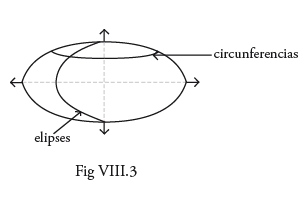
\includegraphics{./tex_imgs/repslatex-img48.png}

~~El eje fundamental del sistema de referencia es el eje de rotación, el
plano fundamental es el que es normal al eje de revolución y pasa por el
centro del elipsoide, corta al mismo en una sección circular llamada
ecuador elipsóidico, cuyo radio es el semieje mayor de la elipse ``a''.

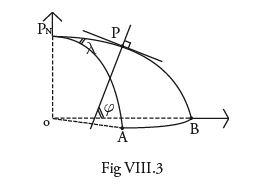
\includegraphics{./tex_imgs/repslatex-img49.png}

~~Dado un punto P cualquiera sobre el elipsoide, es posible trazar un
plano tangente a la superficie que contenga a P, la recta que pasa por P
y es perpendicular al plano tangente, se denomina ``normal al
elipsoide''.

~~La latitud elipsóidica \({\varphi }\) o geodésica del punto P sobre el
elipsoide se define como el ángulo entre la normal en P y el ecuador
elipsóidico; se mide de 0 a 90, positivo al Norte y negativo al Sur.

~~La longitud elipsóidica \({\lambda }\) o geodésica del punto P es el
ángulo diedro entre el meridiano que pasa por P y otro definido como
origen; se mide de 0 a 180, positivo hacia el este y negativo hacia el
Oeste.

~~El acimut elipsóidico A es el ángulo entre dos planos, ambos contienen
a la normal al elipsoide en P: uno contiene a los polos y el otro a la
dirección considerada.

VIII.3.- CORTES NORMALES.

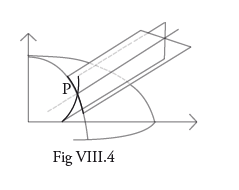
\includegraphics{./tex_imgs/repslatex-img50.png}

~~Dada una superficie cualquiera, se puede considerar en un punto P
sobre la misma un haz de infinitos planos que contienen a la normal a la
superficie en P. Dichos planos son llamados planos normales y determinan
\textbf{secciones normales}. Las secciones normales al elipsoide son las
que se obtienen de la intersección de la superficie con los planos que
contienen la normal al elipsoide. Existen infinitas secciones normales
en todo punto P del elipsoide; todas son elipses en el caso del
elipsoide de revolución. Las secciones se caracterizan por acimut. Así
habrá una sección de acimut cero: llamada de sección meridiana, y otra
de acimut de 90°: la sección normal al meridiano.

\hypertarget{radios-de-curvatura}{%
\subsection{Radios de Curvatura}\label{radios-de-curvatura}}

~~Los radios de curvatura que son de interés son los de las secciones
normales al elipsoide, y si existen infinitas secciones normales hay
infinitos radios de curvatura.

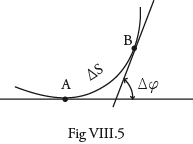
\includegraphics{./tex_imgs/repslatex-img51.png}

~~Dada una curva plana se define como curvatura media, al cociente entre
el ángulo que forman las tangentes a la curva en los puntos extremos del
arco y la longitud del arco; por lo tanto:

\[{C_{{m}}=\frac{\Delta \varphi }{\Delta S}}\]

\[\Delta S >> AB\]

Se llama curvatura en un punto A, al límite:

\[C = \lim_{\Delta S \to 0} \frac{\Delta \Phi}{\Delta S} = \frac{d \Phi}{dS}\]

En una circunferencia, la curvatura será:

\[\frac{d\varphi}{dS}=\frac{d\varphi}{R\,d\varphi}\]

\[C=\frac{1}{R}\]

La curvatura es la inversa del radio. Se llama en general radio de
curvatura en un punto de una curva dada, al valor recíproco de la
curvatura dada en el punto; su valor está dado por:

\[{R=\frac{\left(1+y'^{{2}}\right)^{{\frac{3}{2}}}}{y\text{{\textquotesingle}{\textquotesingle}}}=\frac{\left(1+\left(\frac{dy}{dx}\right)^{{2}}\right)^{{\frac{3}{2}}}}{\frac{d^{{2}}y}{dx^{{2}}}}}\]

De los infinitos radios de curvatura de las secciones normales en un
punto del elipsoide, habrá uno de valor máximo y otro de valor mínimo,
llamados radios principales de curvatura, y son:

~~M: el radio de curvatura del meridiano o sección meridiana.
Corresponde a acimut cero, y es el menor.

~~N: el radio de curvatura de la sección normal al meridiano o primer
vertical. Corresponde a acimut de noventa grados y es el radio mayor.

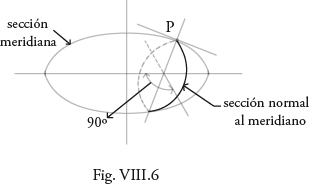
\includegraphics{./tex_imgs/repslatex-img54.png}

~~Estos radios de curvatura tienen un papel importante no solo en la
Geodesia, sino además en la Cartografía, en las deducciones de las
expresiones de la proyección Gauss-Kruger, por lo tanto el propósito es
determinar los valores de M y N en función del elipsoide, es decir se
sus parámetros y de la posición del punto sobre el mismo, es decir de
sus coordenadas.

~~Tanto M y N son función de los parámetros del elipsoide y de la
latitud solamente, ya que sus secciones meridianas son iguales.

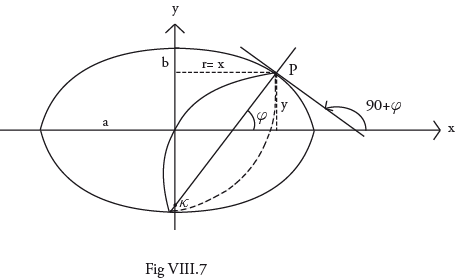
\includegraphics{./tex_imgs/repslatex-img55.png}

~~Se parte de la ecuación de la elipse meridiana y la del radio de
curvatura. En la elipse meridiana (Fig. VIII.7), ``a'' es el radio del
ecuador y ``b'' el radio polar. Sea P un punto cualquiera sobre la
elipse meridiana, el ángulo que forma la normal en P con el eje mayor es
la latitud \({\varphi }\). Trazando la tangente en el punto P, ésta
forma con el eje de las x el ángulo (90+ \({\varphi }\)). Tanto x e y
pueden considerarse como funciones de una única variable \({\varphi }\),
que es la que interesa en Geodesia y Cartografía. Se puede imaginar el
punto P moviéndose sobre la elipse desde el ecuador hasta el polo; la
latitud varía de 0 a 90, x disminuye de ``a'' a cero, e y crece de cero
a ``b''. Si x e y son funciones de la latitud, también lo son sus
derivadas, las que expresadas en función de la latitud se introducen en
la ecuación del radio de curvatura para encontrar M y N.

~~El radio de curvatura de la sección meridiana M es:

\[{M=\frac{a^{{2}}\cdot b^{{2}}}{\left[a^{{2}}\cdot \text{cos}^{{2}}\left(\varphi \right)+b^{{2}}\cdot sen^{{2}}\left(\varphi \right)\right]^{{\frac{3}{2}}}}}\]

se puede expresar también en función de la excentricidad:

\[{M=\frac{a^{{2}}\cdot \left(1-e^{{2}}\right)}{\left[1-e^{{2}}\cdot sen^{{2}}\left(\varphi \right)\right]^{{\frac{3}{2}}}}}\]

~~Para calcular el radio de curvatura de la sección normal al meridiano,
se establece la ecuación de la elipse correspondiente a esa sección y se
determina el radio de curvatura en el punto que interesa, llegando a las
siguientes expresiones:

\[{N=\frac{a}{\left[1-e^{{2}}\cdot sen^{{2}}\left(\varphi \right)\right]^{{\frac{1}{2}}}}}\]

\[{N=\frac{a^{{2}}}{\left[a^{{2}}\cdot \text{cos}^{{2}}\left(\varphi \right)+b^{{2}}\cdot sen^{{2}}\left(\varphi \right)\right]^{{\frac{1}{2}}}}}\]

~~Se demuestra además que el radio de un paralelo cualquiera de latitud
\({\varphi }\); ver fig VIII.7:

\[{r=N\cdot \text{cos}\left(\varphi \right)}\] Por lo tanto:

\[{N=\frac{r}{\text{cos}\left(\varphi \right)}}\] de donde N es el
segmento PK de la Figura VIII.7.

~~Para algunas deducciones puede ser necesario que los radios de
curvatura se expresen en función de la segunda excentricidad; se
determina que:

\[{M=\frac{a^{{2}}}{b\cdot \left[1+e'^{{2}}\cdot \text{cos}^{{2}}\left(\varphi \right)\right]^{{\frac{3}{2}}}}}\]

\[{N=\frac{a^{{2}}}{b\cdot \left[1+e'^{{2}}\cdot \text{cos}^{{2}}\left(\varphi \right)\right]^{{\frac{1}{2}}}}}\]

Los valores en el polo se encuentran haciéndolo \({\varphi =\text{90}}\)
y se obtiene:

\[{M=N=\frac{a^{{2}}}{b}}\] En el ecuador \({\varphi =0}\), se tiene
que:

\[{M=a\cdot \left(1-e^{{2}}\right)}\] \[{N=a}\] donde M es menor que N;
se evidencia que N es siempre mayor que M, llegándose a igualar en el
polo.

~~Se deduce también que el radio de curvatura de una sección normal de
acimut cualquiera es igual a:

\[{R_{{A}}=\frac{M\cdot N}{M\cdot sen^{{2}}\left(A\right)+N\cdot \text{cos}^{{2}}\left(A\right)}}\]

~~En muchas aplicaciones geodésicas y cartográficas, es suficientemente
aproximado utilizar una esfera auxiliar que reemplaza al elipsoide, cuya
superficie se adapta lo mejor posible en las proximidades del punto de
interés.

~~Esta esfera tiene un radio, que es el valor medio de todos los radios
de curvatura del elipsoide en un punto; esto es:

\[{R=\frac{1}{\left({}^{\pi }/_{2}\right)}\cdot \overset{{A={}^{\pi }/_{2}}}{\underset{{A=0}}{\int }}{R_{{A}}\cdot dA}}\]
Se demuestra que el radio de la esfera que mejor se adapta es:

\[{R=\sqrt{M\cdot N}}\]

VIII.5.- ARCO DE MERIDIANO ELIPSÓIDICO.

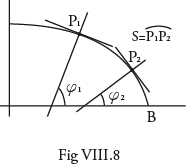
\includegraphics{./tex_imgs/repslatex-img56.png}

~~Si se desea calcular la longitud la longitud de un arco de meridiano
entre dos puntos P1 y P2, teniendo en cuenta que un diferencial de arco
está dado por:

\[{dS=M\cdot d\varphi }\] Se debe integrar dicho elemento entre los
valores de \({\varphi _{{1}}}\) y \({\varphi _{{2}}}\); esto es:

\[{S=\overset{\varphi _{{2}}}{\underset{{\varphi _{{1}}}}{\int }}{M\cdot
d\varphi }}\]

\[{S=\overset{\varphi _{{2}}}{\underset{{\varphi _{{1}}}}{\int}}{\frac{a\cdot \left(1-e^{{2}}\right)}{\left[1-e^{{2}}\cdot sen^{{2}}\left(\varphi \right)\right]^{{\frac{3}{2}}}}\cdot d\varphi }}\]

\[{S=a\cdot \left(1-e^{{2}}\right)\cdot \overset{\varphi _{{2}}}{\underset{{\varphi _{{1}}}}{\int }}{\frac{d\varphi}{\left[1-e^{{2}}\cdot sen^{{2}}\left(\varphi \right)\right]^{{\frac{3}{2}}}}}}\]

Esta integral se resuelve mediante el desarrollo de la serie binomial
del integrando:

\[\begin{matrix}{\left[1-e^{{2}}\cdot sen^{{2}}\left(\varphi \right)\right]^{{-{\frac{3}{2}}}}=1+\frac{3}{2}\cdot e^{{2}}\cdot sen^{{2}}\left(\varphi \right)+\frac{3}{2}\cdot {\frac{5}{4}}\cdot e^{{4}}\cdot sen^{{4}}\left(\varphi \right)+\frac{3}{2}\cdot {\frac{5}{4}}\cdot {\frac{7}{6}}\cdot e^{{6}}\cdot sen^{{6}}\left(\varphi \right)}\hfill\null \\+{\frac{3}{2}}\cdot {\frac{5}{4}}\cdot {\frac{7}{6}}\cdot {\frac{9}{8}}\text{.}\text{.}\text{.}\text{.}\text{.}\text{.}\text{.}\text{.}\text{.}\text{.}\text{.}\text{.}\text{.}\text{.}\text{.}\text{.}\text{.}\text{.}\text{.}\hfill\null \end{matrix}\hfill\]

la cual se debe multiplicar por \({d\varphi }\) y ejecutar la
integración término por término, pero antes de proceder a la
interpretación, se reemplazan las potencias del seno de la latitud en
funciones trigonométricas múltiplos de \({\varphi }\), como se indica a
continuación:

\[{sen^{{2}}\left(\varphi
\right)=\frac{1}{2}-\frac{1}{2}\cdot \text{cos}^{{2}}\left(\varphi
\right)}\] \[{sen^{{4}}\left(\varphi
\right)=\frac{3}{8}-\frac{1}{2}\cdot \text{cos}^{{2}}\left(\varphi
\right)+\frac{1}{8}\cdot \text{cos}^{{4}}\left(\varphi \right)}\]
\[{sen^{{6}}\left(\varphi
\right)=\frac{5}{\text{16}}-\frac{\text{15}}{\text{32}}\cdot
\text{cos}^{{2}}\left(\varphi \right)+\frac{3}{\text{16}}\cdot
\text{cos}^{{4}}\left(\varphi \right)-\frac{1}{\text{32}}\cdot
\text{cos}^{{6}}\left(\varphi \right)}\] \[{sen^{{8}}\left(\varphi
\right)=\frac{\text{35}}{\text{128}}-\frac{7}{\text{16}}\cdot
\text{cos}^{{2}}\left(\varphi \right)+\frac{7}{\text{32}}\cdot
\text{cos}^{{4}}\left(\varphi \right)-\frac{1}{\text{16}}\cdot
\text{cos}^{{6}}\left(\varphi \right)+\frac{1}{\text{128}}\cdot
\text{cos}^{{8}}\left(\varphi \right)}\] Estos últimos valores se
reemplazan en la (VIII.10), y quedan multiplicados por los factores
\({\frac{3}{2}\cdot e^{{2}}}\),
\({\frac{3}{2}\cdot {\frac{5}{4}}\cdot e^{{4}}}\), etc. Se agrupan luego
según los cosenos múltiplos de la latitud, y para abreviar conviene
escribir:

\[{A=1+\frac{3}{4}\cdot
e^{{2}}+\frac{\text{45}}{\text{64}}e^{{4}}+\frac{\text{175}}{\text{256}}\cdot
e^{{6}}+\frac{\text{11025}}{\text{16384}}\cdot
e^{{8}}\text{.}\text{.}\text{.}\text{.}\text{.}\text{.}\text{.}\text{.}\text{.}\text{.}\text{.}\text{.}\text{.}}\]

\[{B=-\left[\frac{3}{4}\cdot
e^{{2}}+\frac{\text{15}}{\text{16}}e^{{4}}+\frac{\text{525}}{\text{512}}\cdot
e^{{6}}+\frac{\text{2205}}{\text{2048}}\cdot
e^{{8}}+\text{.}\text{.}\text{.}\text{.}\text{.}\text{.}\text{.}\text{.}\text{.}\text{.}\text{.}\text{.}\text{.}\right]}\]

\[{C=\overset{}{{}}\overset{}{{}}\overset{}{{}}\overset{}{{}}\overset{}{{}}\left[\frac{\text{15}}{\text{64}}e^{{4}}+\frac{\text{105}}{\text{256}}\cdot e^{{6}}+\frac{\text{2205}}{\text{4096}}\cdot e^{{8}}+\text{.}\text{.}\text{.}\text{.}\text{.}\text{.}\text{.}\text{.}\text{.}\text{.}\text{.}\text{.}\text{.}\right]}\]

\[{D=\overset{}{{}}\overset{}{{}}\overset{}{{}}\overset{}{{}}\overset{}{{}}\overset{}{{}}\overset{}{{}}\overset{}{{}}\overset{}{{}}-\left[\frac{\text{35}}{\text{512}}\cdot
e^{{6}}+\frac{\text{315}}{\text{2048}}\cdot
e^{{8}}+\text{.}\text{.}\text{.}\text{.}\text{.}\text{.}\text{.}\text{.}\text{.}\text{.}\text{.}\text{.}\text{.}\right]}\]

\[{E=\overset{}{{}}\overset{}{{}}\overset{}{{}}\overset{}{{}}\overset{}{{}}\overset{}{{}}\overset{}{{}}\overset{}{{}}\overset{}{{}}\overset{}{{}}\overset{}{{}}\overset{}{{}}\overset{}{{}}\overset{}{{}}\overset{}{{}}+\left[\frac{\text{315}}{\text{16384}}\cdot
e^{{8}}+\text{.}\text{.}\text{.}\text{.}\text{.}\text{.}\text{.}\text{.}\text{.}\text{.}\text{.}\text{.}\text{.}\right]}\]

Reemplazando en (VIII.10) se tiene que:

\[{\left[1-e^{{2}}\cdot sen^{{2}}\left(\varphi
\right)\right]^{{\frac{-3}{2}}}=A+B\cdot \text{cos}\left(2\varphi
\right)+C\cdot \text{cos}\left(4\varphi \right)+D\cdot
\text{cos}\left(6\varphi \right)+E\cdot \text{cos}\left(8\varphi
\right)+\text{.}\text{.}\text{.}\text{.}}\]

Multiplicando por \({a\cdot \left(1-e^{{2}}\right)\cdot d\varphi}\), y
teniendo en cuenta la (VIII.9), se tiene que:

\[{S=a\cdot \left(1-e^{{2}}\right)\overset{\varphi
_{{2}}}{\underset{{\varphi _{{1}}}}{\int }}{\left[A+B\cdot
\text{cos}\left(2\varphi \right)+C\cdot \text{cos}\left(4\varphi
\right)+D\cdot \text{cos}\left(6\varphi \right)+E\cdot
\text{cos}\left(8\varphi
\right)+\text{.}\text{.}\text{.}\text{.}\right]}{?d\varphi }}\]

Integrando esta última expresión se obtiene el arco de meridiano
elipsóidico entre dos valores de latitud dados; por lo tanto:

\[{S=a\cdot \left(1-e^{{2}}\right)\cdot \left(A+\frac{B}{2}\cdot
sen\left(2\varphi \right)+\frac{C}{4}\cdot
sen\left(4\varphi \right)+\frac{D}{6}\cdot
sen\left(6\varphi \right)+\frac{E}{8}\cdot
sen\left(8\varphi
\right)+\text{.}\text{.}\text{.}\text{.}\right)|_{{\varphi
_{{1}}}}^{\varphi _{{2}}}}\]

En esta expresión el valor de la latitud que acompaña a A se debe
introducir en radianes.

En caso que se desee introducir la latitud en grados sexagesimales, hay
que agregar en el primer término del paréntesis el factor
\({\frac{1}{\rho _{{o}}}}\), siendo el \({\rho _{{o}}}\) el número de
grados contenidos en un radián.

Para simplificar aún más la última expresión, se puede escribir:

\[{\alpha =a\cdot \left(1-e^{{2}}\right)\cdot A}\]

\[{\beta =\frac{a}{2}\cdot \left(1-e^{{2}}\right)\cdot B}\]

\[{\gamma =\frac{a}{4}\cdot \left(1-e^{{2}}\right)\cdot C}\]

\[{\delta =\frac{a}{6}\cdot \left(1-e^{{2}}\right)\cdot D}\]

\[{\varepsilon =\frac{a}{8}\cdot \left(1-e^{{2}}\right)\cdot E}\]

con lo cual la expresión del arco se transforma en:

\[S=\alpha \varphi + \beta sen (2\varphi) + \gamma sen (4\phi) + \delta sen (6\varphi) + \epsilon sen (8\varphi) + ... |_{\Phi1}^{\Phi2}\]
~~~Por medio de las expresiones vistas se calculan de una vez, para un
determinado elipsoide, las constantes \({\alpha ,\beta ,\gamma ,\delta
,\varepsilon }\), las que dependen únicamente del semieje mayor y de la
excentricidad de la elipse meridiana. Luego con la expresión (VIII.11)
se puede calcular un arco de meridiano entre dos valores de latitud
cualesquiera.

~~En Cartografía existen dos arcos de meridiano de especial interés,
como se verá más adelante. Éstos son el arco de meridiano desde el
ecuador hasta un punto de latitud cualquiera y el arco de meridiano
desde el polo sur al punto de la latitud considerada, valores éstos que
forman parte de las expresiones de las coordenadas de U.T.M. y
Gauss-Kruger, respectivamente.

~~En el primer caso, \(\varphi_1=0\) , la expresión se transforma en:

\[S=\alpha \varphi + \beta sen (2\varphi) + \gamma sen (4\phi) + \delta sen (6\varphi) + \epsilon sen (8\varphi)\]

En el segundo \(\varphi_1=90°=\frac{\varpi}{2}\), se tiene que la se
transforma en:

\[S=\alpha \left( \varphi + \frac{\varpi}{2} \right) + \beta sen (2\varphi) + \gamma sen (4\phi) + \delta sen (6\varphi) + \epsilon sen (8\varphi)\]

recordando que el valor de la latitud en el primer término debe
expresarse en radianes.

VIII.6.- ARCO DE PARALELO ELIPSÓIDICO.

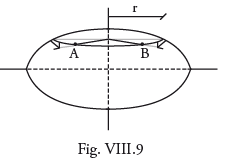
\includegraphics{./tex_imgs/repslatex-img64.png}

Dado que el elipsoide es de revolución, los paralelos son
circunferencias. Un elemento de arco de paralelo está dado por:

\[dp=r\,d\lambda=N\,cos(\varphi)\,d\lambda\]

El valor de un arco de paralelo entre las longitudes \(\lambda_1\) y
\(\lambda_2\) está dado por:

\[AB=N\,cos(\varphi)\,(\lambda_2-\lambda_1)\]

IX.1.- MÓDULO DE DEFORMACIÓN LINEAL

Siguiendo la misma secuencia teórica del capítulo IV, se desarrollan las
expresiones del módulo de deformación lineal, pero considerando como
figura de la tierra el elipsoide.

\includegraphics{./tex_imgs/repslatex-img77.png}

~~Sean dos puntos sobre el elipsoide, P y Q, de coordenadas
\({P(\varphi ,\lambda )}\) y \({Q(\varphi +d\varphi ,\lambda
+d\lambda )}\). Los arcos de paralelo y meridiano elementales son
respectivamente:

\[{d\rho =N\cdot \text{cos}\left(\varphi \right)\cdot
d\lambda }\] \[{dm=M\cdot d\varphi }\] De donde la distancia elemental
es:

\[ dL=\sqrt{\left(M\, d\varphi \right)^{2}+\left[N\, \text{cos}\left(\varphi \right)\, d\lambda \right]^{2}} \]
(IX.1)

El área del rectángulo individual es igual:

\[dS=M \, N \, \text{cos}\left(\varphi \right) \, d\varphi \, d\lambda\]
(IX.2)

Y el acimut del elemento distancia dL es:

\[\text{tg}\left(A\right)=\frac{N \, \text{cos}\left(\varphi \right) \, d\lambda}{M \, d\varphi}\]
(IX.3)

Las expresiones de las imágenes de dL, dS y A en el plano son las mismas
vistas en (IV.1).

Por lo tanto el módulo de deformación es:

\[{m_{{l}}=\frac{dl}{dL}}\] Reemplazando en la (IV.5) y la (IX.1) se
tiene:

\[{m_{{l}}^{{2}}=\frac{\left(dx\right)^{{2}}+\left(dy\right)^{{2}}}{\left(M\cdot
d\varphi \right)^{{2}}+\left[N\cdot \text{cos}\left(\varphi
\right)\cdot d\lambda \right]^{{2}}}}\] De la misma manera que se dedujo
en la (IV.26):

\[{m_{{l}}^{{2}}=\frac{E\cdot \left(d\varphi \right)^{{2}}+G\cdot
\left(d\lambda \right)^{{2}}+2\cdot F\cdot d\varphi
\cdot d\lambda }{\left(M\cdot d\varphi
\right)^{{2}}+\left[N\cdot \text{cos}\left(\varphi \right)\cdot
d\lambda \right]^{{2}}}}\] Siendo el mismo razonamiento que en (IV.27)

\[{m_{{l}}^{{2}}=\frac{E}{M^{{2}}}\cdot
\text{cos}^{{2}}\left(A\right)+G\cdot
{\frac{sen^{{2}}\left(A\right)}{\left[N\cdot
\text{cos}\left(\varphi \right)\right]^{{2}}}}+F\cdot
{\frac{sen\left(2A\right)}{M\cdot N\cdot
\text{cos}\left(\varphi \right)}}}\] (IX.4)

De esta última expresión se desprende que el módulo de deformación
lineal es en elipsoide es función de la latitud y del acimut, y por
supuesto de la ley de representación.

~~Para hallar el máximo y mínimo de la expresión (IX.4) se diferencia el
módulo de deformación lineal en función del acimut, y se iguala la
derivada a cero, como se efectuó en (IV.28); en este caso se arriba a la
siguiente expresión:

\[{tg\left(2A\right)=\frac{2\cdot F\cdot
M\cdot N\cdot \text{cos}\left(\varphi \right)}{\left[E\cdot N\cdot
\text{cos}\left(\varphi \right)-G\cdot M\right]}}\] (IX.5)

~~Para encontrar las expresiones de los módulos de deformación lineal
según los meridianos y según los paralelos, se debe hacer en la (IX.4)
A=0 y A=90, respectivamente y se obtiene:

\[{m_{{l}}^{{m}}=\frac{\sqrt{E}}{M}}\] (IX.6)

\[{m_{{l}}^{{p}}=\frac{\sqrt{C}}{N\cdot \text{cos}\left(\varphi \right)}}\]
~~A continuación se desarrollarán las proyecciones geodésicas de mayor
uso en la práctica: estereográfica polar, Mercator y Cónica de Lambert.

~~En capítulo aparte las proyecciones Gauss-Kruger, y su aplicación en
la Argentina y la proyección U.T.M. (Universal Transversal Mercator)
serán desarrolladas, por lo particular de su planteo y por la amplia
difusión de ambas proyecciones en todo el mundo.

X.2.- PROYECCIÓN GAUSS-KRÜGER.

~~Dados dos puntos sobre el elipsoide infinitamente próximos (figura
IX.2), ambos vienen caracterizados por sus coordenadas geográficas
latitud y longitud. Teniendo en cuenta que ambos puntos son
infinitamente próximos, se puede considerar que la parcela elipsóidica
que abarcan no tienen curvatura, es decir que es un plano que se
denominará ``z'', es decir que la superficie elemental \({\left(d\varphi
,d\lambda \right)}\) se supone plana.

~~Ambos puntos tienen su imagen plana, cuyas posiciones se caracterizan
por sus coordenadas planas ortogonales X e Y en la carta, que se
denominará plano de las ``u''.

Se trata de establecer la relación funcional entre la superficie
elipsóidica elemental con la correspondiente superficie plana, con la
condición que la representación sea conforme. De acuerdo con lo
anteriormente expuesto se hace uso de la funciones de variable compleja
porque ellas satisfacen dicha condición.

~~Se forman para cada plano las variables complejas:

\[{z=\varphi +i\lambda }\]

\[{u=X+iY}\] Ambas variables están ligadas por la función de variable
compleja:

\[{u=f\left(z\right)}\]

O sea:

\[{X+iY=f\left(\varphi +i\lambda
\right)}\] (X.7)

Formando la variable compleja \({\varphi +i\lambda }\) no se ha elegido
la misma unidad lineal para la parte real y la parte imaginaria de la
variable. Si se incrementan en 1'' por ejemplo la latitud y longitud, el
arco de meridiano es siempre el mismo para cualquier latitud, no así el
arco de paralelo que disminuye a medida que la longitud aumenta.

~~Los arcos de meridiano y paralelo en el elipsoide son respectivamente:

\[{dm=M\cdot d\varphi }\] \[{dp=N\cdot \text{cos}\left(\varphi
\right)\cdot d\lambda }\] En la esfera:

\[{dm=R\cdot d\varphi }\] \[{dp=R\cdot \text{cos}\left(\varphi
\right)\cdot d\lambda }\] Por lo tanto el arco de paralelo disminuye de
acuerdo con el coseno de la latitud. Por ejemplo 1'' en el ecuador y a
60 de latitud le corresponden los siguientes arcos de meridiano y
paralelo:

\[dm\left(0{}^{\circ}\right)=\text{30}m\]
\[{dp\left(0{}^{\circ}\right)=\text{30}m}\]

\[dm\left(\text{60}{}^{\circ}\right)=\text{30}m\]

\[dp\left(\text{50}{}^{\circ}\right)=\text{15}m\]

~~Es decir, que sobre la superficie elipsóidica considerada plana, no se
tienen cuadrados elementales sino rectángulos elementales, por no
producir el mismo incremento lineal sobre el elipsoide, incrementos
iguales en latitud y longitud. Si:

\[{d\varphi =d\lambda }\] Las unidades lineales en el sentido de la
latitud y la longitud están en la relación:

\[{\frac{dp}{dm}=\frac{M}{N\cdot \text{cos}\left(\varphi \right)}}\]

~~Para igualar los arcos de meridiano y paralelo se sustituye la latitud
`` \$\{\emph{φ} \}\$'' por una nueva variable ``q'' llamada latitud
isométrica, contada también a partir del ecuador de manera que el
elemento de meridiano se exprese:

\[{M\cdot d\varphi =N\cdot \text{cos}\left(\varphi \right)\cdot
dq}\] Porque se desea que para iguales incrementos de latitud isométrica
y longitud:

\[{dq=d\lambda }\] Se produzcan iguales incrementos lineales sobre
meridianos y paralelos. Por lo tanto:

\({dq=\frac{M\cdot d\varphi }{N\cdot
\text{cos}\left(\varphi \right)}}\) (X.8)

En el caso de una esfera sonde M=N=R se tiene que:

~~\({dq=\frac{d\varphi
}{\text{cos}\left(\varphi \right)}}\) (X.8')

Si por ejemplo \({dq=d\lambda
=1\text{{\textquotesingle}{\textquotesingle}}}\), en la latitud de 60 se
tiene que:

\[{dm=R\cdot d\varphi =R\cdot
\text{cos}\left(\varphi \right)\cdot
dq=\text{15}m}\] \[{dm=R\cdot d\varphi =R\cdot
\text{cos}\left(\varphi \right)\cdot
dq=\text{15}m}\] Integrando las (X.8) y (X.8'):

\[{q=\text{ln}\left[tg\left(\text{45}\text{{\textdegree}+}\frac{\varphi
}{2}\right)\right]-\frac{e}{2}\cdot \text{ln}\left(\frac{1-e\cdot
sen\left(\varphi \right)}{1+e\cdot
sen\left(\varphi \right)}\right)}\]
\[{q=\text{ln}\left[tg\left(\text{45}\text{{\textdegree}+}\frac{\varphi
}{2}\right)\right]-\frac{e}{2}\cdot \text{ln}\left(\frac{1-e\cdot
sen\left(\varphi \right)}{1+e\cdot
sen\left(\varphi \right)}\right)}\]

\end{document}
